\secnumbersection{DEFINICIÓN DEL PROBLEMA}

\subsection{CONTEXTO}

Durante años hemos necesitado encontrar el camino para llegar desde un lugar a otro, la velocidad con la que se obtiene esta información puede ser de gran ayuda en casos como encontrar el camino a un lugar con un GPS o encontrar un camino optimizado para un robot.
Problema del camino más corto es un problema de la teoría de grafos que quiere encontrar un camino con una característica menor, en nuestro caso es tiempo de viaje.
En casos donde el algoritmo no es lo suficientemente rápido se pueden usan atajos para obtener soluciones menos óptimas pero que son mas rápidas de obtener.

\subsection{PROBLEMA}

\textit{Pathfinding}, es una rama del problema del camino mas corto, se basa en buscar el camino entre dos puntos en un espacio representado computacionalmente(Ver figura \ref{fig:example}). Se busca una lista de posiciones por las cuales tenga que pasar el agente\footnote{Entidad que tiene que moverse por el tablero.} de tal modo que se simplifique el movimiento a saltos entre posiciones como en un tablero o movimientos simples como lineas rectas que pueda seguir el agente.

\begin{figure}[h]
\centering
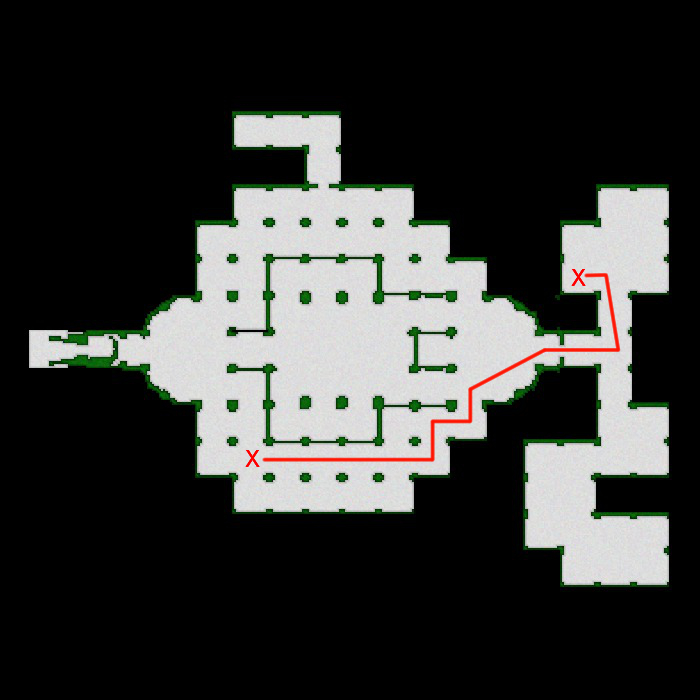
\includegraphics[width=0.8\textwidth]{example}
\caption{\label{fig:example} Ejemplo de \textit{pathfinding}} Fuente: \textit{Dragon Age: Origins}\cite{bioware2009pathfinding}.
\end{figure}

\subsection{DIFERENCIAS}

\subsubsection{TABLERO}

Dependiendo del tipo de tablero en el que tiene encontrar un camino se encuentran distintos problemas, estos se separan en:

\begin{itemize}
    \item Estático: El único movimiento en el tablero es el agente que esta buscando el camino, este es el caso mas simple porque no se tiene que ajustar el \textit{pathfinding} durante el movimiento.
    \item Dinámico: Existen cambios en el tablero provocados por otras entidades o otros efectos. En este caso el problema es que el camino encontrado con anterioridad puede parar de ser funcional de un momento a otro y buscar el camino completamente después de cada movimiento es demasiado costoso.
\end{itemize}

También existen problemas donde se puede encontrar el camino para distintos tipos de agentes que se relacionan diferente con los distintos tipos de terreno, por ejemplo, agentes que puedan desplazarse sobre el agua no tienen que preocuparse de esquivarla.

\subsubsection{VISIBILIDAD}

Otro punto a considerar es el conocimiento previo del tablero y la visibilidad que se tiene de este, si el tablero es conocido, se pueden usar algoritmos que permiten optimizar el \textit{pathfinding} con procesamiento previo, estos se separan en:

\begin{itemize}
    \item Conocimiento total del tablero: El agente conoce el tablero y tiene visión de este en cada momento.
    
    \item Conocimiento del tablero pero visibilidad reducida: El agente tiene alguna especie de cámara o visión periférica por lo cual conoce los cambios en el tablero que están cerca de el.
    
    \item Conocimiento reducido: No hay conocimiento del tablero y este se genera con la visión del agente mientras se esta moviendo.
\end{itemize}

\subsubsection{MOVIMIENTO}

El movimiento del agente puede ser variable dependiendo del terreno por lo cual puede variar el tiempo o el coste\footnote{En juegos con turnos, los agentes tienen una cantidad de puntos para sus movimientos que se reducen dependiendo del terreno por el que caminan}. También el movimiento puede separarse en:

\begin{itemize}
    \item Discreto: En juegos con tablero se usa este tipo de movimiento porque las posiciones posibles están dadas por enteros, como en el ajedrez.
    
    \item Continuo: En el trabajo de robótica y en juegos en tiempo real se usan movimientos continuos, para encontrar el camino el mundo continuo se reduce a un sistema discreto y luego con ese sistema se puede crear el movimiento continuo.
\end{itemize}

\subsubsection{TAMAÑO}

Cuando tienes que mover distintos agentes dentro de un tablero, pueden existir agentes que ocupan mas espacio que otros por lo cual sus caminos tienen que poder contenerlos. Casos como unidades que ocupan 1 celda del tablero y otras que ocupan 4 puedes ser mas complicados de tratar en un solo grafo.


\subsection{GRAFOS}

La representación que se usara en la memoria son grafos, un conjunto de nodos unidos por arcos que permiten relacionar a estos. Estos nodos son las posibles posiciones en el espacio y los arcos representan las formas de movimiento entre ellos.
Los arcos llevan un valor agregado que nos permite saber cuanto cuesta el movimiento desde un punto a otro, en un tablero de cuadrados existen 4 u 8 formas de movimiento dependiendo de como sea la decisión de diseño(Ver figura \ref{fig:example2}). Los movimientos cardinales tienen un coste 1 y los diagonales tienen un coste $ \sqrt{2} $.
Se explicara mas a fondo en el Marco Conceptual.


\begin{figure}[h]
\centering
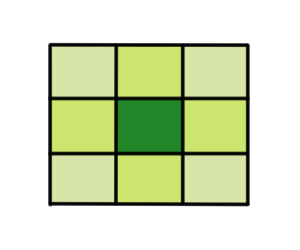
\includegraphics[width=0.5\textwidth]{example2}
\caption{\label{fig:example2} Ejemplo de movimiento entre Nodo central, sus cuatro direcciones cardinales y las diagonales en colores diferentes.} Fuente: Propio.
\end{figure}

\subsection{ENFOQUE}

En esta memoria nos centraremos en el problema de \textit{pathfinding} en juegos en tiempo real, por lo cual los dos problemas principales que se enfrentan son:

\begin{itemize}

    \item Tiempo: En los juegos normalmente se le permite un tiempo a la búsqueda de caminos de algunos mili segundos para no entorpecer el funcionamiento del resto de las funciones del juego por lo cual la velocidad de el algoritmo se vuelve imperativa para que la calidad del juego no sea afectada.
    
    \item Calidad: Dentro del tiempo que es posible ocupar se tiene que entregar la mejor solución posible de tal modo que los agentes no tomen caminos que podrían ser denominados de poco humano para los jugadores.
    
\end{itemize}

Además nos estamos enfocado en mapas auto generados\footnote{Creados en el momento que se inicia la partida} no podemos usar pre-procesamiento para obtener un aumento de velocidad en el \textit{pathfinding}, por lo cual nos enfrentamos a un problema que no permite ocupar pre-procesamiento directamente. 

\subsection{OBJETIVO DE LA SOLUCIÓN}


\subsubsection{OBJETIVOS GENERALES}


\subsubsection{OBJETIVOS ESPECÍFICOS}


\begin{enumerate}
    \item  
    \item
    \item
\end{enumerate}